\subsection{Anaheim network, equilibrium and predefined regions}\label{app:anaheimsettings}
Both network and demand files are the public Transportation Networks for Research Core Team Anaheim TNTP data \citep{tnfrc2024transportation}. The network header supplies free-flow times in minutes and capacities in vehicles per hour; all roads use the published BPR coefficient 0.15 and power 4. We use $t_e(F_e)=t_e^0[1+0.15(F_e/c_e)^4]$ and TSTT marginal weight $t_e^0[1+0.75(F_e/c_e)^4]$. The six study OD demands, ranked by descending base demand and then lexicographic OD, are $(4,2)$: 2106.7, $(1,2)$: 1365.9, $(2,4)$: 1271.4, $(3,2)$: 1237.9, $(25,4)$: 1232.4, $(25,2)$: 1232.3 vehicles per hour. They move jointly from 0.8 to 1.2 times base demand; all remaining positive demands stay at their published base values and retain endogenous route choice. Every OD uses ten loopless free-flow shortest routes from Yen's algorithm. Ties within $10^{-12}$ minutes are resolved by lexicographic edge-index sequence in the TNTP road order. Nodes 1--38 are centroids and cannot be intermediate route nodes; the first through node is 39. Logit scale $\theta=1$ minute$^{-1}$ applies to route travel time in minutes.
The edge Newton solver targets maximum loading residual below $10^{-8}$ vehicles per hour, uses at most 80 iterations and backtracking up to 30 halvings per step, and checks the original path loading residual below $10^{-7}$. Implicit derivatives solve the same fixed-point equation. Trapezoidal integration uses equally spaced states, with warm starts from a neighboring saved state. The 41-state refinement reuses all 21 old states and computes only the twenty new midpoints.
The distance-based region construction and fixed progress targets are specified in Section~\ref{sec:anaheim}. The reported range uses every admissible prefix in that family. Same-state mechanisms compare regions chosen nearest the progress targets, using free-flow weights $t^0$ and congestion weights equal to the total-flow TSTT marginal weight minus $t^0$.
\begin{figure}[pos=htbp]\centering
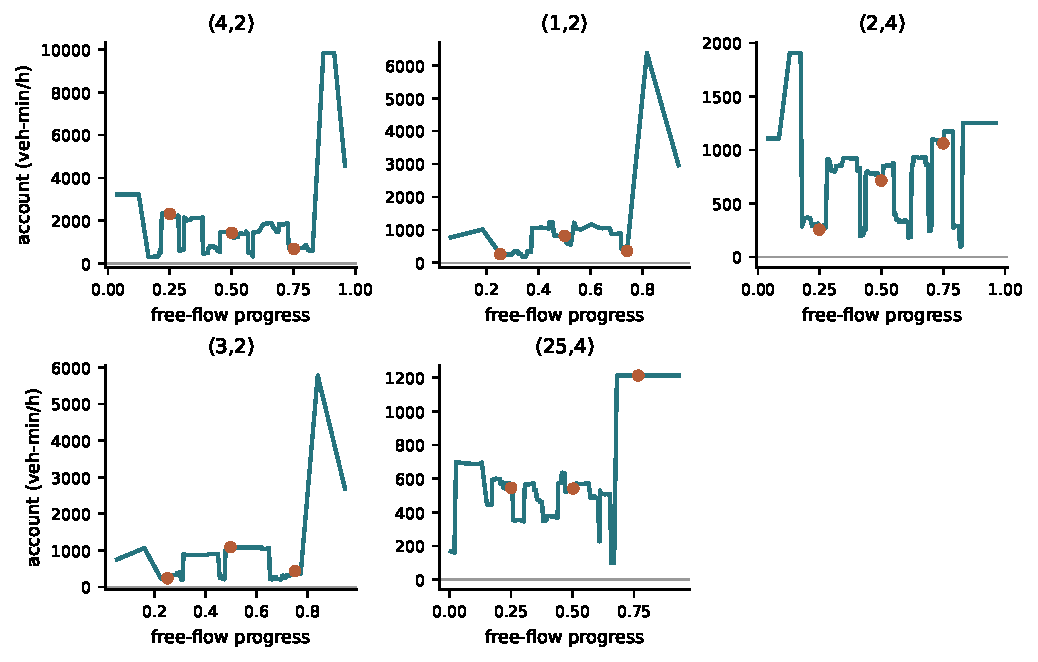
\includegraphics[width=0.99\linewidth]{../figures/fig_v106_anaheim_rest.pdf}
\caption{Anaheim spatial response profiles of the remaining five study
queries over the distance-based families: the account versus free-flow
progress along each query's own OD direction, with ochre dots marking
the three prespecified positions. All stay positive; family ranges span
roughly one to one and a half orders of magnitude.}\label{fig:anaheimrest}
\end{figure}
